\documentclass[xetex,mathserif,serif]{beamer}
\usepackage{polyglossia}
\setdefaultlanguage[babelshorthands=true]{russian}
\usepackage{minted}
\usepackage{tabu}

\useoutertheme{infolines}

\usepackage{fontspec}
\setmainfont{FreeSans}
\newfontfamily{\russianfonttt}{FreeSans}

\definecolor{links}{HTML}{2A1B81}
\hypersetup{colorlinks,linkcolor=,urlcolor=links}

\usepackage{forest}
\usetikzlibrary{arrows}

\tabulinesep=0.7mm

\title{Сортировки}
\author[Юрий Литвинов]{Юрий Литвинов \newline \textcolor{gray}{\small\texttt{yurii.litvinov@gmail.com}}}

\date{28.09.2018}

\begin{document}
	
	\frame{\titlepage}
	
	\begin{frame}
		\frametitle{Свойства сортировок}
		\begin{itemize}
			\item Работают над любыми контейнерами данных
			\item Есть понятие ``ключ''
			\item Устойчивость --- сохраняется ли взаимное расположение элементов с одинаковым ключом
			\item Естественность --- учёт степени отсортированности исходных данных
			\item Внутренняя сортировка --- работает над данными, целиком помещающимися в память
			\item Внешняя сортировка работает над данными на устройствах с последовательным доступом, которые медленнее, чем память
		\end{itemize}
	\end{frame}

	\begin{frame}
		\frametitle{Сортировка вставкой (insertion sort)}
		\begin{columns}
			\begin{column}{0.4\textwidth}
				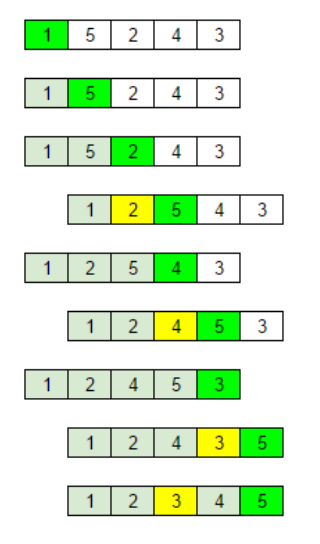
\includegraphics[width=0.8\textwidth]{insertion-sort.png}
			\end{column}
			\begin{column}{0.6\textwidth}
				\begin{itemize}
					\item $O(n^2)$
					\item Устойчива
					\item Естественная ($O(n)$ на отсортированном массиве)
					\item Данные могут приходить постепенно
					\item Позволяет выбрать наибольшие (или наименьшие) $k$ чисел из входного потока
				\end{itemize}
			\end{column}
		\end{columns}
	\end{frame}

	\begin{frame}
		\frametitle{Сортировка Шелла (Shell sort)}
		\begin{columns}
			\begin{column}{0.4\textwidth}
				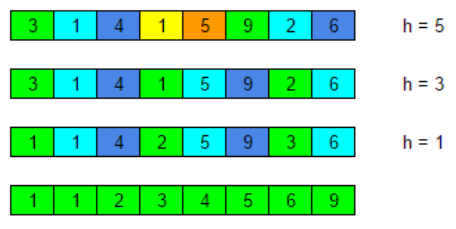
\includegraphics[width=0.8\textwidth]{shell-sort.png}
			\end{column}
			\begin{column}{0.6\textwidth}
				\begin{itemize}
					\item Сортировка вставкой подпоследовательностей в массиве с постепенно убывающим шагом
					\item Элементы ``быстрее'' встают на свои места
					\begin{itemize}
						\item Сортировка вставкой на каждом шаге уменьшает количество инверсий максимум на 1
					\end{itemize}
					\item $O(n * log(n)^2)$ при правильном выборе h
					\item Неустойчива
					\item Легко пишется и довольно быстра
					\begin{itemize}
						\item Не вырождается до квадратичной
					\end{itemize}
				\end{itemize}
			\end{column}
		\end{columns}
	\end{frame}

	\begin{frame}
		\frametitle{Сортировка выбором (Selection sort)}
		\begin{columns}
			\begin{column}{0.4\textwidth}
				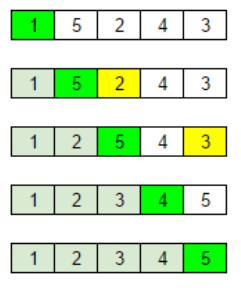
\includegraphics[width=0.8\textwidth]{selection-sort.png}
			\end{column}
			\begin{column}{0.6\textwidth}
				\begin{itemize}
					\item $O(n^2)$
					\item Обычно неустойчива ([$2_a$, $2_b$, $1_a$] -> [$1_a$, $2_b$, $2_a$])
					\item Отсортированность массива ничего не даёт
					\item Меньше всего операций обмена (меньше операций записи, что иногда позитивно)
				\end{itemize}
			\end{column}
		\end{columns}
	\end{frame}

	\begin{frame}
		\frametitle{Быстрая сортировка (qsort)}
		\begin{columns}
			\begin{column}{0.5\textwidth}
				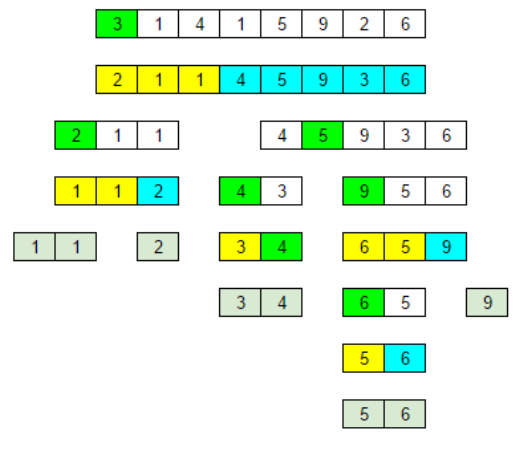
\includegraphics[width=0.8\textwidth]{qsort.png}
			\end{column}
			\begin{column}{0.5\textwidth}
				\begin{itemize}
					\item $O(n * log(n))$, вырождается до $O(n^2)$
					\item Неустойчива
					\item Требует $O(n * log(n))$ дополнительной памяти
					\item Самый быстрый на практике алгоритм сортировки, используется в стандартных библиотеках
					\item Легко пишется (но тяжело отлаживается)
				\end{itemize}
			\end{column}
		\end{columns}
	\end{frame}

	\begin{frame}[fragile]
		\frametitle{Псевдокод}
		\begin{columns}
			\begin{column}{0.5\textwidth}
				\begin{footnotesize}
					\begin{minted}{pascal}
algorithm quicksort(A, lo, hi) is
    if lo < hi then
        p := partition(A, lo, hi)
        quicksort(A, lo, p – 1)
        quicksort(A, p + 1, hi)
					\end{minted}
				\end{footnotesize}
			\end{column}
			\begin{column}{0.5\textwidth}
				\begin{footnotesize}
					\begin{minted}{pascal}
algorithm partition(A, lo, hi) is
    pivot := A[hi]
    i := lo  
    for j := lo to hi – 1 do
        if A[j] ≤ pivot then
            swap A[i] with A[j]
            i := i + 1
    swap A[i] with A[hi]
    return i
					\end{minted}
				\end{footnotesize}
			\end{column}
		\end{columns}
		\vspace{1cm}
		Нерекурсивная реализация --- через стек, в котором хранятся границы сортируемых кусков массива
	\end{frame}

	\begin{frame}
		\frametitle{Сортировка кучей (пирамидальная, heapsort)}
		\begin{columns}
			\begin{column}{0.6\textwidth}
				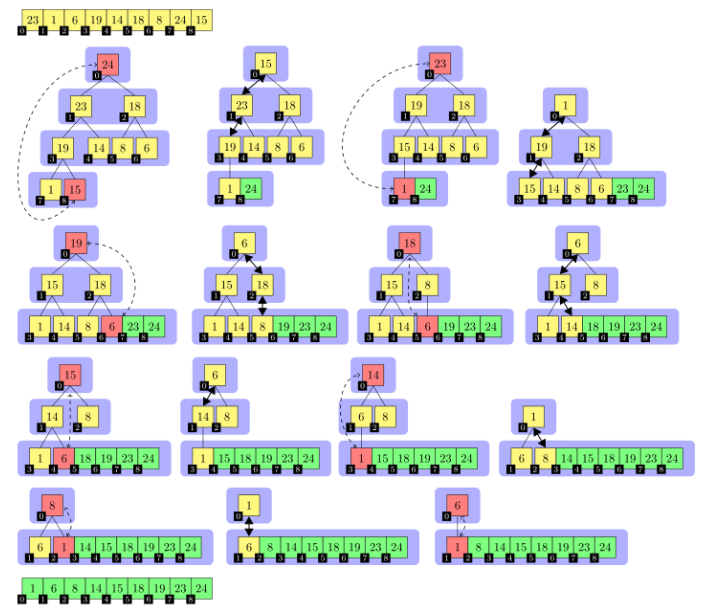
\includegraphics[width=0.95\textwidth]{heapsort.png}
			\end{column}
			\begin{column}{0.4\textwidth}
				\begin{itemize}
					\item $O(n * log(n))$, не вырождается
					\item Не требует дополнительной памяти
					\item Неустойчива
					\item Требует произвольного доступа к памяти
					\item Сложна в реализации
				\end{itemize}
			\end{column}
		\end{columns}
	\end{frame}

	\begin{frame}
		\frametitle{Двоичный поиск}
		\begin{columns}
			\begin{column}{0.5\textwidth}
				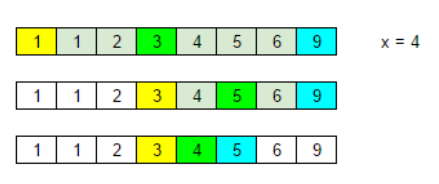
\includegraphics[width=0.8\textwidth]{binary-search.png}
			\end{column}
			\begin{column}{0.5\textwidth}
				\begin{itemize}
					\item Находит элемент в массиве за $O(log(n))$
					\item Легко напутать с индексами и уйти в бесконечный цикл
				\end{itemize}
			\end{column}
		\end{columns}
	\end{frame}

\end{document}

